\documentclass[xcolor=table, compress, %
handout
]{beamer}

\usepackage{appendixnumberbeamer}
\usetheme{Pittsburgh}
%\usepackage{beamerthemesplit}
\usecolortheme{beaver}
\setbeamercolor{navigation symbols}{fg=black, fg=gray}
\setbeamercolor{structure}{fg=gray}
\setbeamercolor{alerted text}{fg=darkred}
\resetcounteronoverlays{exx}

\usepackage{setspace}
\usepackage{relsize}
\usepackage{pgfpages}
\usepackage{graphicx}
\usepackage{booktabs}
\usepackage{subfigure}	% mehrere Bilder in einer figure-Umgebung
\usepackage{marvosym} %Radioaktiv-Zeichen
\usepackage[ngerman, english]{babel}
%\usepackage{beamerthemesplit}

%\usepackage{lmodern,textcomp}

\usepackage{fontspec}
\setromanfont{CMU Serif}
\setsansfont{CMU Sans Serif}
\setmonofont{CMU Typewriter Text}

\usepackage{tikz}
\usepackage{tikz-qtree}
\usepackage{tikzducks}

\usepackage{tipa}
\usepackage{verbatimbox} % Muss bei beamer als \begin{frame}[fragile] gekennzeichnet werden


%% biblatex-Optionen und Gestaltung der Bibliographie
\usepackage[style=authoryear-comp, natbib=true, maxcitenames=3, backend=biber]{biblatex}
\bibhang1em
%\usepackage[babel, english=quotes]{csquotes}
\DeclareFieldFormat{postnote}{#1}%--> kein S. in Zitaten
\DeclareFieldFormat{multipostnote}{#1}%--> kein S. in Zitaten
\renewcommand*{\postnotedelim}{\addcolon\addspace}%%--> : statt , in Zitaten
\DeclareFieldFormat{pages}{#1} %%--> kein S. in Bibliographie
\renewcommand*{\bibpagespunct}{\addcolon\addspace} %%--> : in Bibliographie statt ,
\bibliography{BibliographieNegation.bib}

\usepackage[babel, german=quotes]{csquotes}
\usepackage{ragged2e}

%Linguistik-Pakete%
\usepackage{expex}
\usepackage{gb4e}
\usepackage{xcolor}

\mode<handout>{
\setbeamertemplate{footline}[frame number]
}

\lingset{
    aboveglftskip=0pt,
    belowglpreambleskip=0pt,
    belowpreambleskip=0pt,
    extraglskip=0pt,
    Everyex={\parskip=0pt},
}

%neue Kommandos Oliver%
\newcommand{\qu}[1]{„#1“}
\newcommand{\qufs}[1]{,#1‘}
\newcommand{\tsub}[1]{\textsubscript{#1}}
\newcommand{\tsup}[1]{\textsuperscript{#1}}
\newcommand{\tuple}[1]{$\langle$#1$\rangle$}
\newcommand{\blau}[1]{{\color{blue} #1}}
\newcommand{\rot}[1]{{\color{red} #1}}
\def\newblock{\hskip .11em plus.33em minus.07em}
\let\eachwordone=\sf  % Schriftart bei Glossen bleibt bei Übergängen gleich
\let\eachwordtwo=\sf  %
\newcommand{\oldoe}{$\stackrel{\textsf{\tiny e}}{\textsf{o}}$}

%\setbeamercolor{alerted text}{fg=red}

\newcommand*{\ballref}[1]{%
    \begin{pgfpicture}{-1ex}{-0.65ex}{1ex}{1ex}
    \usebeamercolor[fg]{item projected}
    {\pgftransformscale{1.75}\pgftext{\normalsize\pgfuseshading{bigsphere}}}
    {\pgftransformshift{\pgfpoint{0pt}{0.5pt}}
      \pgftext{\usebeamerfont*{item projected}\ref{#1}}}
  \end{pgfpicture}}%
  
  % Edh und Thorn
\DeclareTextSymbolDefault{\dh}{T1}
\DeclareTextSymbolDefault{\th}{T1}

% Makro für arbiträre übergeschriebene Buchstaben
\newcommand{\supr}[2]{$\stackrel{\text{\smaller#2}}{\text{#1}}$}

\selectlanguage{ngerman}

\title[Loss of the MHG bipartite negation marker \textit{ne ... niht}]{\bf{The loss of the MHG bipartite negation marker \textit{ne ... niht}}}
\subtitle{Diachronic and diatopic variation in ReM and CAO}
\author[Daniel Hrbek and Oliver Schallert]{%
Daniel Hrbek\inst{1} \and Oliver Schallert\inst{2}}
\institute{%
\inst{1} Osnabrück University %\\ Institut für Germanistik \\ 

\href{mailto:daniel.hrbek@uni-osnabrueck.de}{\texttt{daniel.hrbek@uni-osnabrueck.de}}
\and
\inst{2} Ludwig Maximilian University of Munich %\\ Institut für Deutsche Philologie \\ 

\href{mailto:oliver.schallert@lmu.de}{\texttt{oliver.schallert@lmu.de}}
}

\date{2 July 2022}

\pgfdeclareimage[width=2.5cm]{logo}{LMU-Logo.png}
% Logo Uni Osnabrück ergänzen
 \pgfdeclareimage[width=3.75cm]{pogo}{UOS-R.jpg} 
% \pgfdeclareimage[width=3.75cm]{pogo}{UOS-SW.jpg} 
% \pgfdeclareimage[width=3.75cm]{pogo}{UOS-SWR.png} 
\titlegraphic{\vspace{-0.2cm}\pgfuseimage{pogo}\hspace{0.5cm}\pgfuseimage{logo}}

\begin{document}

\begin{frame}
\thispagestyle{empty}
\titlepage
\end{frame}



\begin{frame}{Roadmap}

\tableofcontents[sections={1-2}]

\end{frame}

\begin{frame}{Roadmap}

\tableofcontents[sections={3-5}]


\end{frame}

\begin{frame}{Acknowledgements}

\begin{itemize}
\item \alert{Julia Hertel} (née Schüler) (Saarland University) for sharing work from her PhD thesis with us.
\item \alert{Carsten Becker} (University of Marburg) for the fruitful work on MHG charters we have done together.
\end{itemize}

\end{frame}


\section{Point of departure}

\begin{frame}{Point of departure}

\pex[] \label{a}
\a
\begingl
\gla die \textbf{ne}mugin iz uernemen//
\glb they NEG=could it hear//
\glft (Wiener Physiologus 149va,5)//
\endgl
\a
\begingl
\gla er\textbf{ne} wil dich \textbf{nit} lazen//
\glb he=NEG wants you NEG let//
\glft (Rolandslied 0a,8969)//
\endgl
\a
\begingl
\gla Sí	ſprachen \textbf{niht} an dem hilígen tag//
\glb they talked NEG on the sacred day//
\glft  (Oberaltaicher Evangelistar 25ba,37)//
\endgl
\xe

\end{frame}

\begin{frame}{Point of departure}


\begin{itemize}
\item In all Old Germanic languages, we find a preverbal negation particle \textit{ni}/\textit{ne} that derives from PTG \textit{*ni} (cf. \citealt{Eythorsson1995}, \citealt{Eythorsson2002}):
\end{itemize}

\pex
\a
\begingl
\gla ni was wul\th ag \textup{(Gothic)}//
\glb \textsc{NEG} was glorious//
\glft (2nd Letter Corinthians 3,10)//
\endgl
\a
\begingl
\gla ni láz thir nan ingángan \textup{(OHG)}//
\glb \textsc{NEG} let you him escape//
\glft (Otfrid IV 37,11)//
\endgl
\a
\begingl
\gla út \th ú ne komir / órum hǫllum frá //
\glb out you \textsc{NEG} come {} our.\textsc{DAT.PL} hall.\textsc{DAT.PL} from//
\glft \textup{(Old Norse) (Vaf\th rú\dh nismál 7)} //
\endgl
\xe

\end{frame}

\begin{frame}{Point of departure}

\begin{itemize}
\item \citet[690]{Grimm1890} already noted that the early Germanic dialects are strikingly similar in terms of their negation patterns:
\end{itemize}

\begin{quote}
\raggedright
NI war die ursprüngliche und wahre negation; in der goth sprache hat sie noch den weitesten spielraum, in den übrigen nimmt sie allmählich ab, wiewohl auf verschiedne weise; heutzutag ist sie vor dem verbo überall verschwunden und den partikeln gewichen, die anfangs bloss zu ihrer verstärkung hinter das verbum gestellt wurden und zum theil mit ihr selbst zusammengesetzt sind. 
\end{quote}

\end{frame}



\section{Negation: diachronic aspects}
\subsection{\textit{Jespersen's Cycle}}


\begin{frame}{Negation: diachronic aspects}
\framesubtitle{\textit{Jespersen's Cycle}}
\textit{Jespersen's Cycle} consists of three stages which can be observed:

\begin{itemize}
    \item \alert{Stage I:} the single preverbal element OHG \textit{ni} gets (phonologically) weakened $\rightarrow$ MHG \textit{ne/en}
    \item \alert{Stage II:} now weakened \textit{ne} is insufficient to express negation on its own and is therefore strengthened by an additional element MHG \textit{niht} ($<$ OHG \textit{niouuiht} ‘nothing’) $\rightarrow$ \alert{bipartite negation marker} \textit{ne ... niht}
    \item \alert{Stage III:} the original element falls victim to complete loss $\rightarrow$ MHG \textit{niht} expresses (sentential) negation on its own
\end{itemize}

\end{frame}

\begin{frame}{Negation: diachronic aspects}
\framesubtitle{\textit{Jespersen's Cycle}}

\begin{figure}[h]
\centering
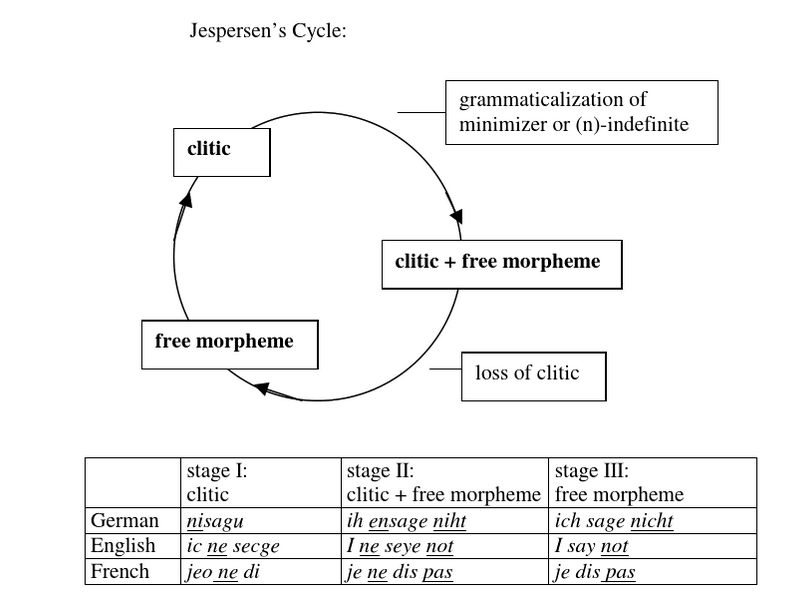
\includegraphics[width=8cm]{Jespersen.png}
\caption{\textit{Jespersen's Cycle} (\citealt[15]{jaeger08})}
\end{figure}


\end{frame}

\begin{frame}{Negation: diachronic aspects}
\framesubtitle{Previous studies}

\begin{itemize}
    \item For a long time, \textit{Jespersen's Cycle} was regarded to hold for West Germanic in its entirety.
    \item In particular, it also applies to Low German (\citealt{Breitbarth2014}).
    \item Therefore, MHG was assumed to represent stage II: \textit{ne ... niht} as the main strategy of negation.
    \item However, recent studies for MHG (\citealt{jaeger08,Pickl2017}) reveal that the situation in MHG is significantly more complex.
\end{itemize}

\end{frame}

\begin{frame}{Negation: diachronic aspects}
\framesubtitle{Previous studies}

\begin{itemize}
    \item Jägers (\citeyear{jaeger08}) data suggest that MHG finished \textit{Jespersen's Cycle} at the end of the 13th century – at the latest.
    \item Pickl’s (\citeyear{Pickl2017}) study on sermons support Jäger’s findings for Upper German $\rightarrow$ \textit{niht} as the main negation strategy already by 1200.
    \item However, \citet{witzenhausen19} (\textit{ne} only) and \citet{schueler16}/\citet{HertelimErscheinen}, who analyzed MHG charters (incl. Western Central German dialects) both oberve a high amount of areal variation.
\end{itemize}

\end{frame}

\begin{frame}{Negation: diachronic aspects}
\framesubtitle{Previous studies}

\begin{center}
\begin{tabular}{l l l l}
\toprule
 & \textbf{Bipartite negation} & \textbf{Single \textit{niht}} & \textbf{Total}\\
\hline
Cologne & 64 (94,1\%) & 4 (5,9\%) & 68 (100\%)\\
Regensburg & 6 (5,5\%) & 103 (94,5\%) & 109 (100\%)\\
Zürich & 1 (1,3\%) & 78 (98,7\%) & 79 (100\%)\\
\hline
total & 71 (27,6\%) & 186 (72,4\%) & 256 (100\%)\\
\bottomrule
\end{tabular}
\end{center}
\begin{small}
\begin{center}\smallskip
Table: Variation in sentential negation in MHG charters by 1280 (\citealt[98]{schueler16})\end{center}
\end{small}
\end{frame}


\subsection{Open issues}

\begin{frame}{Negation: diachronic aspects}
\framesubtitle{Open issues}

Previous research shows an unclear picture:

\begin{itemize}
    \item So far, we know that \textit{Jespersen's Cycle} in MHG is subject to strong areal variation.
    \item While UG enters stage III by 1250, CG remains a stage II language by the end of MHG.
    \item Triggers for \textit{Jespersen's Cycle} are still unclear.
    \begin{itemize}
    \item Previous studies suggest syntactic (\citealt{jaeger08,Breitbarth2014}) as well as phonological (\citealt{HertelimErscheinen}) factors.
    \end{itemize}
    \item Both accelerating and inhibiting factors need further investigation.
    
\end{itemize}


\end{frame}


\begin{frame}{Negation: diachronic aspects}
\framesubtitle{Open issues}

We will present results from our two corpus-based studies:

\begin{itemize}
    \item \alert{Referenzkorpus Mittelhochdeutsch}  ‘Reference Corpus of MHG’ (ReM) (1050–1350)
    \item \alert{Corpus der altdeutschen Originalurkunden bis zum Jahre 1300} ‘Corpus of Old German Original Charters until the year 1300’ (CAO)
\end{itemize}

\end{frame}



\section{The empirical base}
\subsection{The ReM}


\begin{frame}{The empirical base}
\framesubtitle{The ReM}

\textbf{Referenzkorpus Mittelhochdeutsch (ReM) :}
    \begin{itemize}
        \item Freely available since 2016, contains texts from the entire Middle High German period (1050–1350) 
        \item $\sim$ 2 millions tokens, PoS-tagged
        \item \alert{balanced} in terms of text genres $\rightarrow$ text type-specific influences can be controlled for.
 \begin{itemize}       
         \item However, in \alert{diachronic and diatopic matters}, the ReM is \textbf{not well-balanced}: Western Central and Eastern Upper German predominate; early texts are scarce.
\end{itemize}
\end{itemize}

{\small
\begin{itemize}
\item[\Pointinghand] East Central dialects are excluded for the most part (relatively young, only small text portions available from this region.
\end{itemize}
}

{\tiny (\citealt{kleinetal16})}

\end{frame}

\begin{frame}{The empirical base}
\framesubtitle{The ReM}

    \begin{itemize}
        \item Although it uses ANNIS3 (\citealt{Krause2016}), the ReM  \alert{lacks syntactic annotations}. $\rightarrow$ limited use for complex syntactic phenomena
        \item Furthermore: Crashes/overloads and occasional errors/bugs 
        \item Queries for negation patterns are possible by indirect means (e.\,g. with distance parameters)
        \item Sample of 501 instances of \textit{ne ... niht} (using \textit{R})
        \item Results presented here taken from \citet{hrbek21}
    \end{itemize}

\end{frame}

\subsection{The CAO}


\begin{frame}{The empirical base}
\framesubtitle{The CAO}

\textbf{Some background:}

\begin{itemize}
\item \textit{Corpus der altdeutschen Originalurkunden} \qu{Corpus of Old German Original Charters until 1300} (CAO) (Wilhelm et al. \citeyear{cao1}–\citeyear{cao5}).
\begin{itemize}
\item Paper edition comprising 5 Volumes plus supplementary materials; completed 2004.
\item An electronic version is available online, however, with only rudimentary search functions. \href{http://tcdh01.uni-trier.de/cgi-bin/iCorpus/CorpusIndex.tcl}{\alert{\tiny{(Link)}}}
\end{itemize}
\end{itemize}

\end{frame}



\begin{frame}{The empirical base}
\framesubtitle{The CAO}


\begin{itemize}
\item Founded by Friedrich Wilhelm (1882–1932);
\item total of 4617 charters; 4289 in German (to a lesser extent also other languages are included, e.\,g. Latin, Middle Dutch).
\item Covers a period from 1200–1300; however, only 0.2\,\% of the materials date before 1250 (\citealt[42]{ganslmayer09}).
\end{itemize}

\begin{table}
\begin{center}
\begin{tabular}{lllll}
\toprule
& until 1279 & 1280–1289 & 1290–1299 & \textbf{Total}\\ 
\cmidrule{1-5}
No. & 621 & 1095 & 2901 & 4617\\
\bottomrule
\end{tabular}
\caption{Extant charters w.\,r.\,t. different decades}
\end{center}
\end{table}

\end{frame}


\begin{frame}{The empirical base}
\framesubtitle{The CAO}

\textbf{Pros and cons:}

\begin{itemize}
\item Issue date and place are usually mentioned;
\item the materials are lexicographically analyzed (i.\,e. lemmatized) via the \textit{Wörterbuch der mittelhochdeutschen Urkundensprache} (WMU).
\item Clear dominance of Upper German regions; see the map on the next slide. 
\end{itemize}

{\small
\begin{itemize}
\item[\Pointinghand] New studies demonstrate its validity for investigating areal variation in MHG (\citealt{beckerschallert21,beckerschallert22a,beckerschallert22b}; \citealt{HertelimErscheinen}).
\end{itemize}
}

\end{frame}


\begin{frame}{The empirical base}
\framesubtitle{The CAO}

	\begin{figure}
		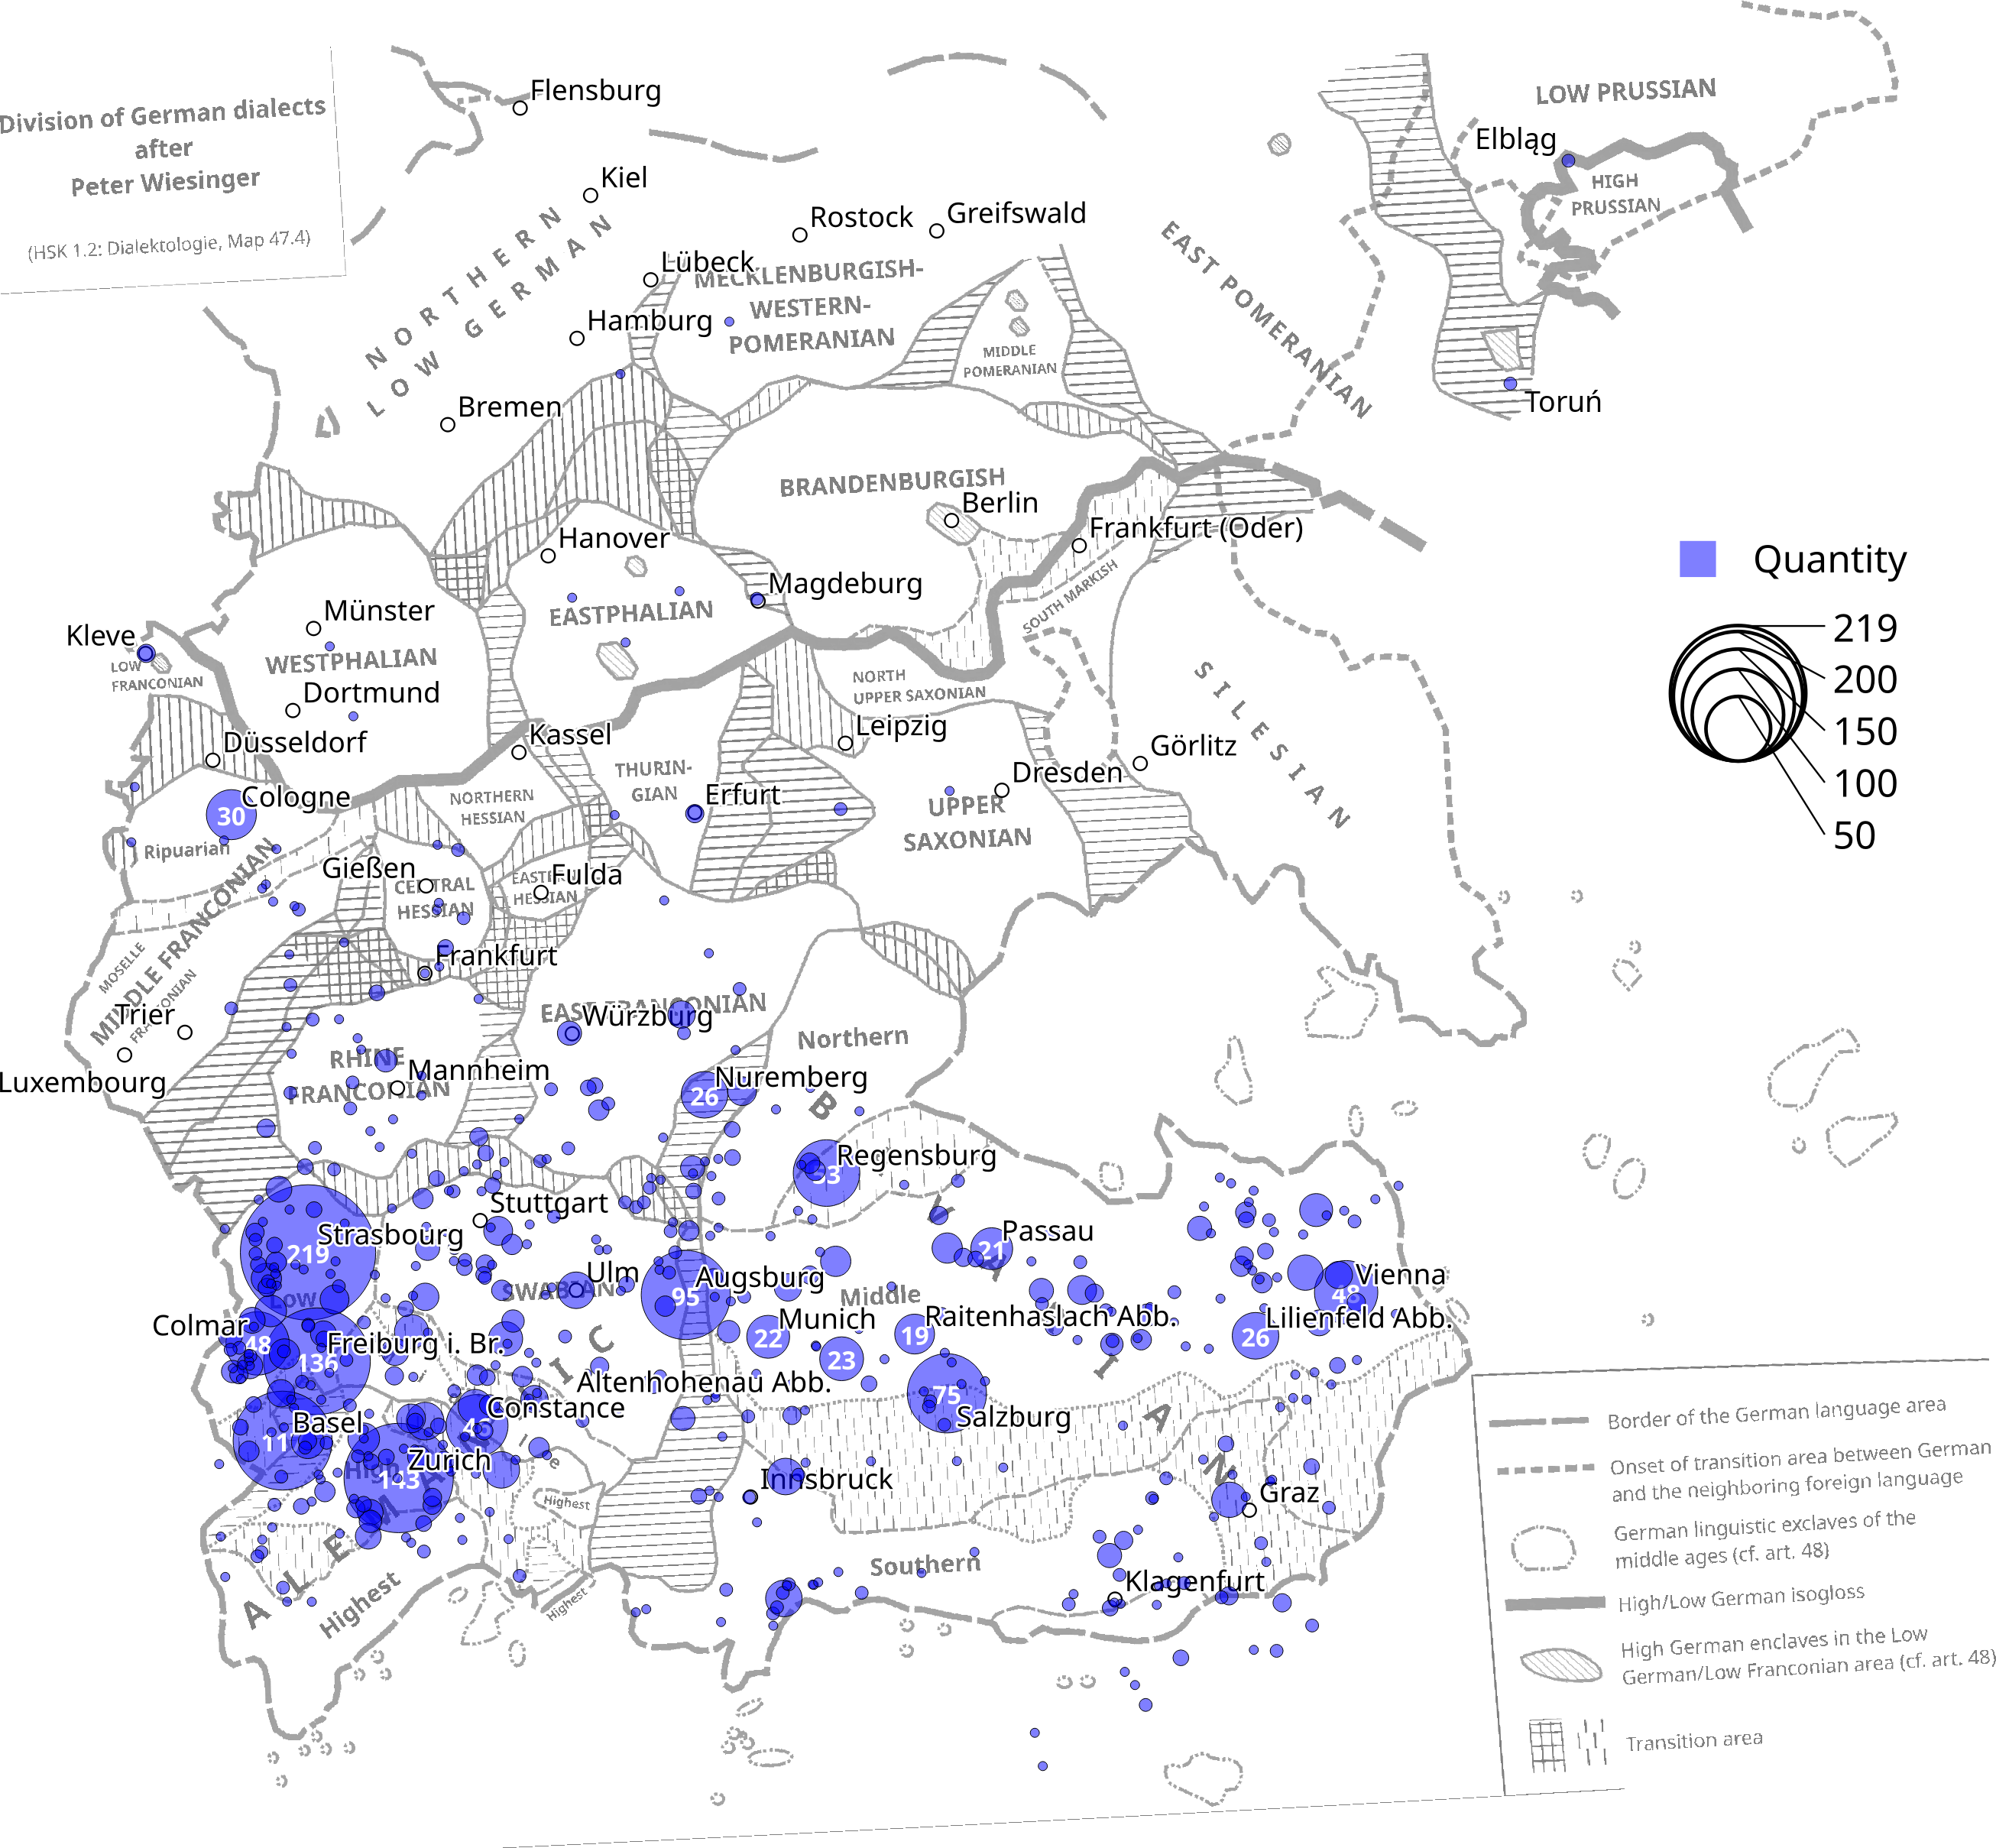
\includegraphics[width=.55\linewidth]{placeunique.png}
		\caption{Number of charters per place \citep[background map adapted
		from][]{wiesinger1983:rede}}
	\end{figure}
\end{frame}


\section{Results}
\subsection{Theoretical background}


\begin{frame}{Results}
\framesubtitle{Theoretical background}

A more detailed look on factors influencing negation:

\begin{itemize}
    \item bipartite negation marker \textit{ne ... niht} mainly attested in Western Central German texts 
    \item early loss (or no use at all) in Upper German texts
    \item early loss in V1 clauses, preservation in embedded clauses (with Vend)
    \item (morphologically) complex verbs with prefixes (as well as participles formed with \textit{ge-}) show an accelerated loss of \textit{ne}/\textit{en}
\end{itemize}

{\tiny (\citealt{behaghel18,Gaertner1977,Pickl2017}; \citealt{schueler16,schueler17}; \citealt{hrbek21})}

\end{frame}


\begin{frame}{Results}
\framesubtitle{Theoretical background}

Prosody-based approach (\citealt{HertelimErscheinen}):

\begin{itemize}
    \item \textit{ne} (reduced variant of OHG \textit{ni} as a weak functional word gets reduced and falls victim to /ə/-deletion quickly.
    \item In V1 clauses with \textit{ne}, the first syllable is unstressed – no trochee possible!
    \begin{itemize}
    \item In MHG, the trochee becomes the preferred foot structure.
    \item e.\,g. wehsele $>$  wechsel\alert{$\varnothing$} ‘exchange’\\
(($\sigma$\textsubscript{s}$\sigma$\textsubscript{r}\alert{$\sigma$\textsubscript{r}})\textsubscript{F})\textsubscript{$\omega$} $>$   (($\sigma$\textsubscript{s}$\sigma$\textsubscript{r}\alert{$\varnothing$})\textsubscript{F})\textsubscript{$\omega$}
    \end{itemize}
    \item The same holds true for prefixed verbs or participles with \textit{ge-}!
    \item VF clauses, on the other hand, preserve the MHG trochee $\rightarrow$ last resort for \textit{ne ... niht}
\end{itemize}

\end{frame}



%
%\section{Involved factores in discussion}
%\begin{frame}{Involved factores in discussion}
%
%Before we take a closer look into our findings, we have to discuss a few phenomena which influenced the deletion of MHG \textit{ne} and \textit{ne ... niht}:
%
%\begin{itemize}
%    \item \textbf{Phonological aspects} which caused \textit{ne} to disappear and
%    \item \textbf{Morphosyntactic aspects} which accelerated or delayed this development.
%\end{itemize}
%
%\end{frame}
%
%\subsection{Phonological aspects}
%
%\begin{frame}{Involved factores in discussion}
%\framesubtitle{Phonological aspects}
%
%During MHG, there are mainly two phonological developments which contradict a long lasting bipartite negation marker:
%
%\begin{itemize}
%    \item \textbf{Reduction of unstressed syllables}: Since late OHG, unstressed syllables with full vowels (such as /a/, /i/, /u/) are slowly reduced to Schwa (/\textipa{@}/).
%    \begin{itemize}
%        \item This development continued until the end of MHG and was subject to a large areal variation.
%        \item While UG was covered quickly and comprehensively, the reduction in CG was significantly delayed.
%    \end{itemize}
%\end{itemize}
%
%\pex
%\a
%OHG \textit{sunna} $\rightarrow$ MHG \textit{sunne}
%\a
%OHG \textit{umbigeban} $\rightarrow$ MHG \textit{umbegeben}
%\xe
%
%\end{frame}
%
%\begin{frame}{Involved factores in discussion}
%\framesubtitle{Phonological aspects}
%
%\begin{itemize}
%    \item \textbf{Schwa (/\textipa{@}/) deletion}: During MHG, Schwa was deleted in reduction syllables and (prosodically) weak functional words (such as particles).
%    \begin{itemize}
%        \item \textit{ne} as a functional word was hit systematically: \textit{ne} $\rightarrow$ \textit{n} $\rightarrow$ \textit{en}
%        \item single /n/ could not survive; a so-called \glqq Stützvokal\grqq{} (\citealt{Nuebling1992}, Paul et al. \citeyear{paul07}) had to be inserted $\rightarrow$ reduction to /\textipa{@}/ and deletion all over again
%        \item From this perspective, MHG \textit{ne} was doomed to death.
%    \end{itemize}
%\end{itemize}
%
%\pex
%\a
%early MHG \textit{kel.be.re} $\rightarrow$ late MHG \textit{kel.ber}
%\a
%OHG \textit{ni} $\rightarrow$ early MHG \textit{ne} $\rightarrow$ \textit{n} $\rightarrow$ late MHG \textit{en}
%\xe
%
%\end{frame}
%
%\begin{frame}{Involved factores in discussion}
%\framesubtitle{Phonological aspects}
%
%\begin{itemize}
%    \item Both developments can be found in the entire MHG area; however, it first started in UG and then slowly spread to CG (\citealt{Triwunatz1913}, \citealt{lindgren53}, \citealt{Klein2005}, \citealt{Buethe-Scheider2017}).
%    \item Completed \textbf{during the 13\textsuperscript{th} century in UG}, but \textbf{not until early 16\textsuperscript{th} century for CG}. 
%    \item[\Radioactivity] Until the development is completely finished, MHG \textit{ne} (as well as \textit{ne ... niht}) remained a \textit{dead man walking}.
%\end{itemize}
%
%\end{frame}
%
%\begin{frame}{Involved factores in discussion}
%\framesubtitle{Phonological aspects}
%
%\begin{itemize}
%    \item One more phonological development – \textbf{fixed metric trochee:} 
%    \item During MHG, the trochee (\textipa{\'xx}) becomes more and more fixed $\rightarrow$ targeted intonation structure
%    \item In order to maintain a trochee in (morphologically) complex words, syllables get deleted:
%\end{itemize}
%
%\pex
%\a
%wehsele   $>$  wechsel\alert{\emptyset} ‘exchange’\\
%(($\sigma$\textsubscript{s}$\sigma$\textsubscript{r}\alert{$\sigma$\textsubscript{r}})\textsubscript{F})\textsubscript{$\omega$} $>$   (($\sigma$\textsubscript{s}$\sigma$\textsubscript{r}\alert{\emptyset})\textsubscript{F})\textsubscript{$\omega$}
%\a
%b. manete $>$ man\alert{\emptyset}te ‘admonished.{\textsc{3SG}}’\\
%(($\sigma$\textsubscript{s}\alert{$\sigma$\textsubscript{r}}$\sigma$\textsubscript{r})\textsubscript{F})\textsubscript{$\omega$} $>$   (($\sigma$\textsubscript{s}\alert{\emptyset}$\sigma$\textsubscript{r})\textsubscript{F})\textsubscript{$\omega$}
%\xe
%
%\end{frame}
%
%\begin{frame}{Involved factores in discussion}
%\framesubtitle{Phonological aspects}
%
%\begin{itemize}
%    \item (Morphologically) simple words (e.g. Sg. Nom.) containing two (or more) syllables lose one (already reduced) syllable
%    \item This is in order to form a trochee in more complex scenarios (e.g. Pl. Gen.).
%    \item This holds true for functional words such as conjuncts and particles.
%\end{itemize}
%%\vspace{-0.5cm}
%%\begin{figure} 
%%\begin{minipage}[t]{0.4755\textwidth}
%%\pex a. swane    $>$ swan ‘swan’\\
%%(($\sigma$\textsubscript{s}$\sigma$\textsubscript{r})\textsubscript{F})\textsubscript{$\omega$}  $>$ 
%%        (($\sigma$\textsubscript{s}\alert{\emptyset})\textsubscript{$\omega$}
%%\end{minipage}
%%\begin{minipage}[t]{0.475\textwidth}
%%\exdisplay b. vnde         $>$ vnd ‘and’ \\
%%(($\sigma$\textsubscript{s}$\sigma$\textsubscript{r})\textsubscript{F})\textsubscript{$\omega$}  $>$ 
%%        (($\sigma$\textsubscript{s}\alert{\emptyset})\textsubscript{$\omega$}
%%\end{minipage} 
%%\end{figure}
%
%\begin{exe}
%\ex swane    $>$ swan ‘swan’\\
%(($\sigma$\textsubscript{s}$\sigma$\textsubscript{r})\textsubscript{F})\textsubscript{$\omega$}  $>$ 
%        (($\sigma$\textsubscript{s}\alert{\emptyset})\textsubscript{$\omega$}
%\ex vnde         $>$ vnd ‘and’ \\
%(($\sigma$\textsubscript{s}$\sigma$\textsubscript{r})\textsubscript{F})\textsubscript{$\omega$}  $>$ 
%        (($\sigma$\textsubscript{s}\alert{\emptyset})\textsubscript{$\omega$}
%\end{exe}
%
%\end{frame}
%
%\subsection{Morphosyntactic aspects}
%\begin{frame}{Involved factores in discussion}
%\framesubtitle{Morphosyntactic aspects}
%Previous studies (\citealt{behaghel18,Gaertner1977,Pickl2017}; \citealt{schueler16,schueler17}, \citealt{hrbek21}) discuss the following points:
%
%\begin{itemize}
%    \item bipartite negation marker \textit{ne ... niht} mainly attested in Western Central German texts ...
%    \item ... and early loss / no use in Upper German texts
%    \item early loss in V1 clauses, preservation in VF clauses
%    \item (morphologically) complex verbs with prefixes (such as participles) tend to accelerate the loss of \textit{ne}/\textit{en}
%\end{itemize}
%
%\end{frame}
%
%\begin{frame}{Involved factores in discussion}
%\framesubtitle{Morphosyntactic aspects}
%
%All of these aspects can be explained with Hertels \citeyear{HertelimErscheinen} prosody based approach:
%
%\begin{itemize}
%    \item \textit{ne} as a weak functional word gets reduced and fells victim to /\textipa{@}/-deletion quickly.
%    \item In V1 clauses with \textit{ne}, the first syllable is unstressed – no trochee possible!
%    \item The same holds true for prefixed verbs (espc. with an reduction syllable like \textit{ge-})!
%    \item VF clauses, on the other hand, preserve the MHG trochee $\rightarrow$ last resort for \textit{ne ... niht}
%\end{itemize}
%
%\end{frame}
%
%\end{document}


\subsection{ReM data}


\begin{frame}{Our results}
\framesubtitle{ReM data}
    
    \begin{itemize}
        \item \textit{ne} underwent a \textit{lexical split} creating a homophone \textit{ne}\textsubscript{2} with exceptive meaning – the ReM does not differentiate between \textit{ne}\textsubscript{1} and \textit{ne}\textsubscript{2}
        \item Ignoring diatopic variation for the time being, our results confirms the findings of \citet{jaeger08} and \citet{Pickl2017}: \textit{ne} gets replaced by \textit{niht} early on.
    \end{itemize}
    
\end{frame}


\begin{frame}{Our results}
\framesubtitle{ReM data}
    
    \begin{figure}[h]
\centering
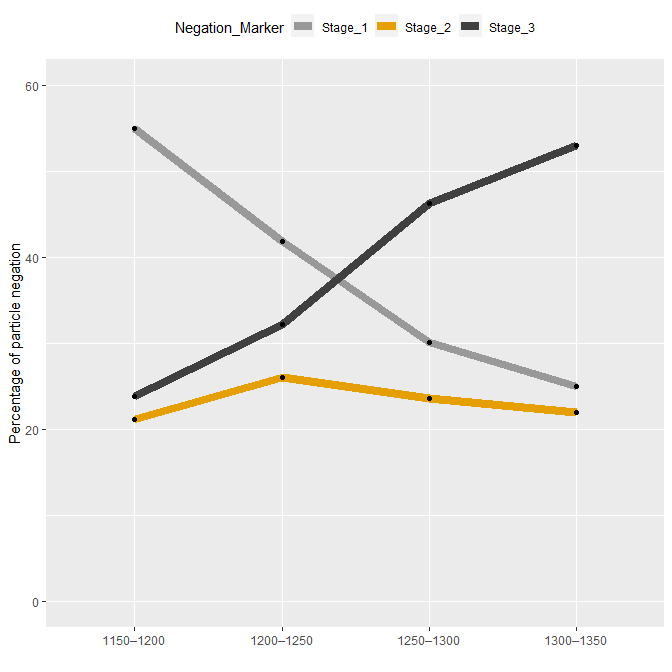
\includegraphics[width=7cm]{Diachron.png}
\end{figure}
    
\end{frame}


\begin{frame}{Our results}
\framesubtitle{ReM data}

\begin{itemize}
\item MHG can be broken down into four major variants: 
\begin{itemize}
\item West and East Upper German
\item West and East Central German (the latter from 1250 onwards)
\end{itemize}
\item Negation patterns vary considerably in the different regions.
\end{itemize}

\end{frame}




\begin{frame}{Our results}
\framesubtitle{ReM data}

\begin{table}
\begin{center}
\begin{tabular}{c c c c c}
\toprule
& \multicolumn{2}{c}{\textbf{East Upper German}} & \multicolumn{2}{c}{\textbf{West Upper German}}   \\
\cmidrule{2-3}
\cmidrule{4-5}
 & \textit{ne \ldots\ niht} & \textit{niht}  & \textit{ne \ldots\ niht}  & \textit{niht}  \\
\hline
1050–1100 & 0 & 0 & 0 & 0 \\
\hline
1100–1150 & 0 & 0 & 0 & 0 \\
\hline
\alert{1150–1200} & \alert{785} & \alert{686} & 47 & 72 \\
\hline
1200–1250 & 154 & 459 & 113 & 115 \\
\hline
1250–1300 & 101 & 611 & 45 & 415\\
\hline
1300–1350 & 59 & 869 & 56 & 310 \\
\hline
\textbf{total} & 1099 & 2625 & 261 & 912\\
\bottomrule
\end{tabular}
\end{center}
\caption{Phase II und III in Upper German }
\end{table}

\end{frame}


\begin{frame}{Our results}
\framesubtitle{ReM data}

\begin{table}
\begin{center}
\begin{tabular}{c c c c c}
\toprule
& \multicolumn{2}{c}{\textbf{East Central German}} & \multicolumn{2}{c}{\textbf{West Central German}}   \\
\cmidrule{2-3}
\cmidrule{4-5}
 & \textit{ne \ldots\ niht} & \textit{niht}  & \textit{ne \ldots\ niht}  & \textit{niht}  \\
\hline
1050–1100 & 0 & 0 & (2) & (2)\\
\hline
1100–1150 & 0 & 0 & (2) & (2)\\
\hline
1150–1200 & 0 & 0 & 101 & 289\\
\hline
1200–1250 & 0 & 0 & 235 & 47\\
\hline
1250–1300 & \alert{113} & \alert{95} & 413 & 199\\
\hline
1300–1350 & \alert{141} & \alert{537} & 676 & 527\\
\hline
\textbf{total} & 254 & 632 & 1427 & 1064\\
\bottomrule
\end{tabular}
\end{center}
\caption{Phase II and III in Central German}
\end{table}
\end{frame}



\begin{frame}{Our results}
\framesubtitle{ReM data}

\begin{itemize}
\item \textbf{Upper German}: 
\begin{itemize} 
\item Rapid change from bipartite to postverbal \textit{niht} between 1150 and 1200. 
\item After 1250, almost every negated clause contains \alert{only \textit{niht}} $\rightarrow$ transition to stage III
\end{itemize}
\textbf{Western Central German}: 
\begin{itemize}
\item \alert{Stable bipartite negation} until the end of the MHG period.
\item The transition from stage II to III negation seems to take place after 1350. \textit{ne ... niht} stays the \textbf{main strategy} for 
\item Fluctuations due to two single texts with an unusal profile (potential influence from West Upper German)
expressing negation.
\end{itemize}
\end{itemize}

{\small
\begin{itemize}
\item[\Pointinghand] Evidence for a stable stage II in MHG!
\end{itemize}
}    

\end{frame}

\begin{frame}{Our results}
\framesubtitle{ReM data}

\textbf{Verb orders with bipartite negation:}
    
\begin{itemize}
\item \alert{V1 clauses are rare} – this is due to prosodic reasons, as we discussed earlier.
\item \alert{V2} is the \alert{most frequent} verb order, but its rate is \alert{decreasing} by comparison with V-end (or V-later).
\item \alert{V-end} seems to have a \alert{preservative effect} (cf. \citealt[245]{behaghel18}).
\end{itemize}

{\small
\begin{itemize}
\item[\Pointinghand] No significant areal variation in this respect (matching the results of \citealt{HertelimErscheinen}).
\end{itemize}
}
    
\end{frame}


\begin{frame}{Our results}
\framesubtitle{ReM data}


\begin{table}
\begin{center}
\begin{tabular}{c c c c}
\toprule
 & \textbf{V1} & \textbf{V2} & \textbf{V-end | V-later}\\
\hline
1150–1200 & 11 & 124 & 16\\
\hline
1200–1250 & 3 & 59 & 21\\
\hline
1250–1300 & 14 & 44 & 48\\
\hline
1300–1350 & 14 & 90 & 57\\ 
\hline
\textbf{gesamt} & 42 & 317 & 142\\
\bottomrule
\end{tabular}
\caption{Bipartite Negation by verb order}
\end{center}
\end{table}

\end{frame}




\subsection{CAO-data}

\begin{frame}{Our results}
\framesubtitle{CAO-data}

\textbf{Phenomena:}

\begin{itemize}
\item Graphical variants of the \alert{clitic negation} norm. \textit{ne, en}, etc.
\begin{itemize}
\item Some variants (not exhaustive) are given in (\ref{klitisch}).
\item Spellings with \textit{i} are indicative of a stage predating phonological weakening.
\end{itemize}
\item \alert{Simple negation} (\textit{en} or \textit{niht}) vs. \alert{discontinuous negation.}
\begin{itemize}
\item Some variants in (\ref{voll}).
\end{itemize}
\end{itemize}


\begin{exe}
\ex  \textit{en(-), ên(-), em-, jn(-), in(-), ien, n-, -n}  (\citealt[1292–1293]{wmu2}) \label{klitisch}
\ex \textit{niht(-), níht, nîht, njcht, n\supr{e}{i}cht, nieht, nivht, n\supr{u}{o}ht, nuht/nvht} (\citealt[1312–1315]{wmu2})  \label{voll}
\end{exe}

\end{frame}

\begin{frame}{Our results}
\framesubtitle{CAO-data}

\textbf{Queries:}

\begin{itemize}
\item We transferred the electronic version of the CAO to an SQL-database. With the aid of the \textit{RNNTagger} (\citealt{schmid2020}), we annotated the data for POS and morphosyntactic information.
\item This enabled us to query directly for the relevant lemmas \textit{he} and \textit{niht} via the tag \texttt{PTKNEG} (STTS tagset).
\item Random sample of 10\,\% of all hits for negation structures (with \textit{R}), manually corrected
\item Graphical variants were annotated exhaustively for vowel quality. 
\end{itemize}

\end{frame}


\begin{frame}{Our results}
\framesubtitle{CAO-data}

\begin{table}
\begin{center}
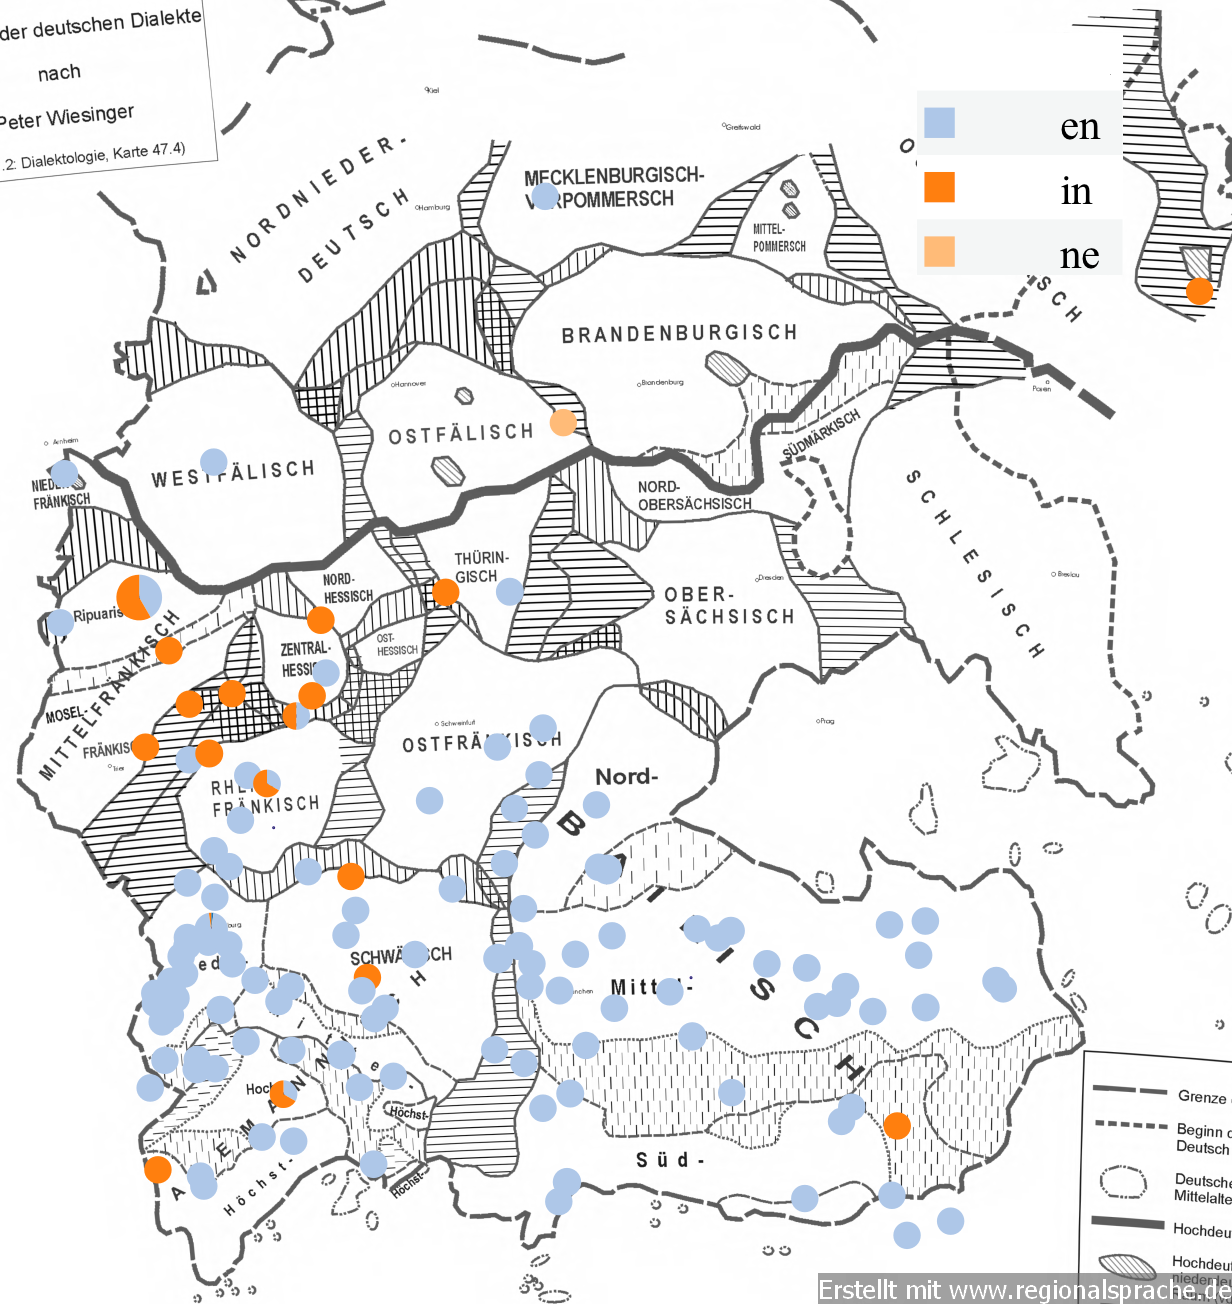
\includegraphics[scale=1]{Graphievarianten.png}
\end{center}
\caption{Graphical variants of the clitic negation}
\end{table}


\end{frame}



\begin{frame}{Our results}
\framesubtitle{CAO-data}

\begin{table}
\begin{center}
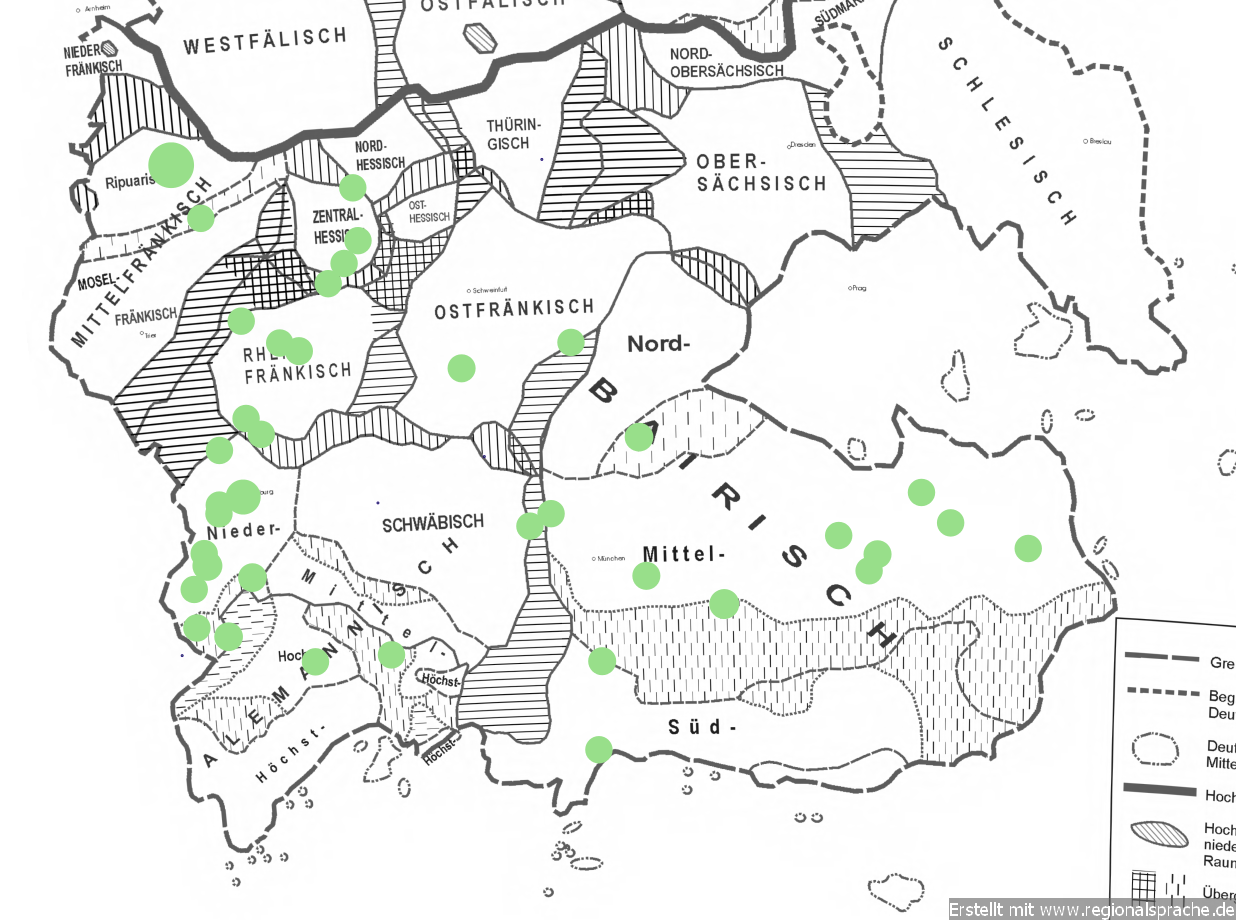
\includegraphics[scale=1.4]{Doppelnegationneu.png}
\end{center}
\caption{Bipartite negation (\textit{ne \ldots\ niht}) in the CAO}
\end{table}


\end{frame}


\begin{frame}{Our results}
\framesubtitle{CAO-data}

\begin{table}
\begin{center}
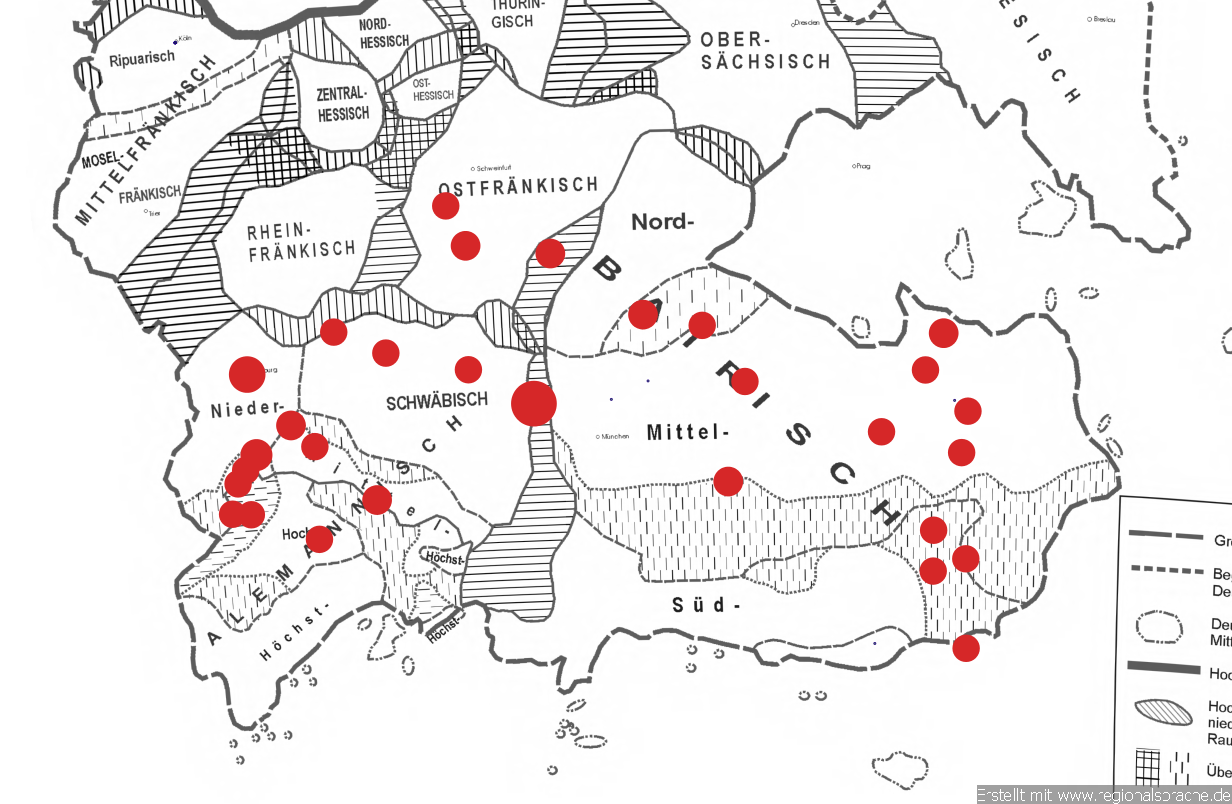
\includegraphics[scale=1.7]{Einfachnegationneu.png}
\end{center}
\caption{Simplex negation (\textit{niht}) in the CAO}
\end{table}


\end{frame}


%\begin{frame}{Our results}
%\framesubtitle{Direction of clitic \textit{ne}}
%
%\begin{itemize}
%    \item In previous literature, it is sometimes mentioned that the preverbal marker (in combination with \textit{niht}) changes its direction when acting like a clitic (e.g. \citealt{Szczepaniak2010}).
%    \item While being a proclitic element in the beginning (6), it can appear as an enclitic later on (7).
%    \item This is most commonly explained with phonotactic reasons (sonority).
%\end{itemize}
%
%\pex[interpartskip=1ex]
%\begingl
%\gla Ein reine wif \textbf{enkan} nýt baz Verdýuen boeſer wive haz//
%\glb a pure woman {\textsc{NEG}}=can \textsc{NEG} better earn evil women hatred//
%\glft M357-G1 0a, 5409–5410 (Das Leben der Gräfin Yolanda von Vianden M)//
%\endgl
%\xe
%\end{frame}
%
%\begin{frame}{Our results}
%\framesubtitle{Direction of clitic \textit{ne}}
%
%\pex[interpartskip=1ex]
%\begingl
%\gla \textbf{ſine} uerſuchtenez an ſi niht mere//
%\glb they={\textsc{NEG}} tried=it without her \textsc{NEG} more//
%\glft M121V-G1 0a, 16768 (Kaiserchronik A, Manuscript V)//
%\endgl
%\xe
%
%\end{frame}
%
%\begin{frame}{Our results}
%\framesubtitle{Direction of clitic \textit{ne}}
%
%\begin{itemize}
%    \item As you will see on the next slide, we couldn't observe such a change.
%    \item However, something did change: \textbf{clitization} (at least on graphematic level) became much more scarce – after 1250, the separately written \textit{ne} is the most frequent variant (8).
%\end{itemize}
%
%\pex[interpartskip=1ex]
%\begingl
%\gla vvan ſie den gotiſ zorn . nivt \textbf{\textipa{\=i}} vorhtin//
%\glb why they the God.{\textsc{GEN}} wrath {} \textsc{NEG} \textsc{NEG} feared//
%\glft M065-G1 62aa, 6–7 (Linzer Entechrist)//
%\xe
%
%\end{frame}
%
%\begin{frame}{Our results}
%\framesubtitle{Direction of clitic \textit{ne}}
%
%\begin{figure}[h]
%\centering
%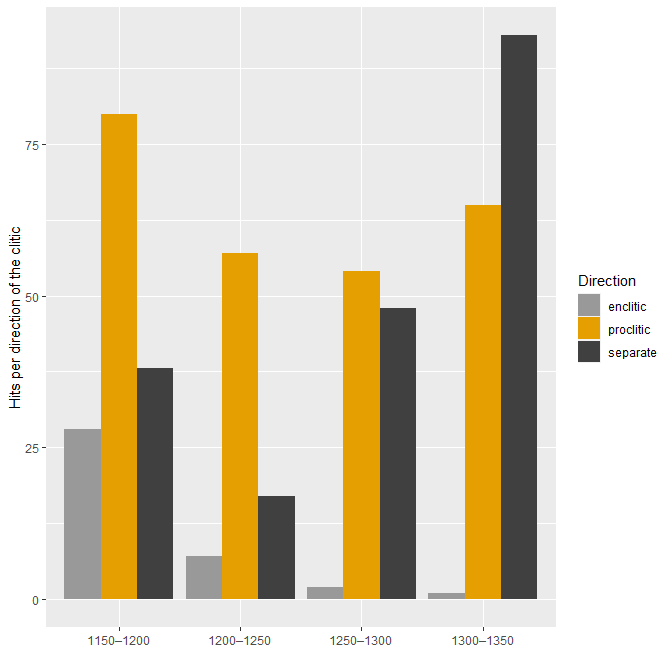
\includegraphics[width=7cm]{Clitic.png}
%\end{figure}
%
%\end{frame}
%
%\begin{frame}{Our results}
%\framesubtitle{Direction of clitic \textit{ne}}
%
%\begin{figure}[h]
%\centering
%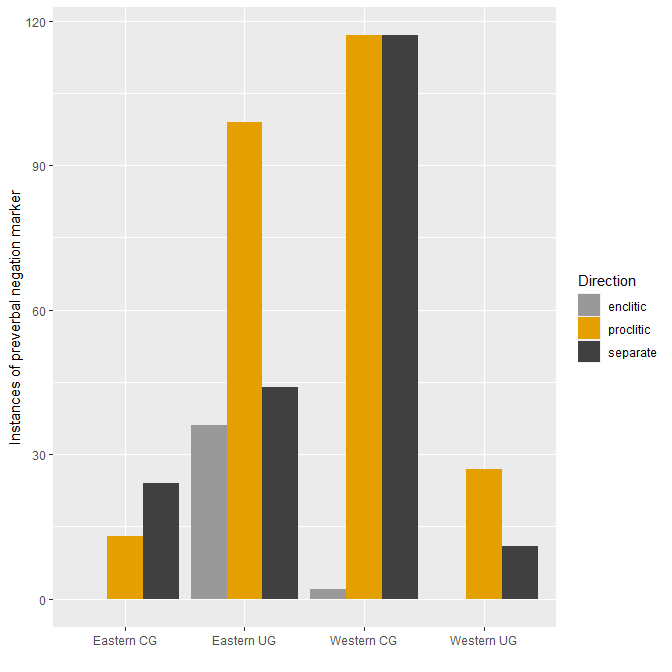
\includegraphics[width=7cm]{CliticD.png}
%\end{figure}
%
%\end{frame}
%
%\begin{frame}{Our results}
%\framesubtitle{Direction of clitic \textit{ne}}
%\renewcommand{\arraystretch}{1.25}
%\begin{center}\resizebox{\textwidth}{!}{%
%\begin{tabular}{c c c c c c c}
%\hline\hline
% & Eastern UG & & & Western CG & & \\
% & Proclitic & Separate & Enclitic & Proclitic & Separate & Enclitic\\
%\hline
%1150–1200 & 72 & 29 & 28 & 3 & 3 & 0\\
%1200–1250 & 10 & 6 & 7 & 16 & 4 & 0\\
%1250–1300 & 11 & 3 & 1 & 2 & 1 & 0\\
%1300–1350 & 6 & 6 & 0 & 6 & 3 & 0\\
%\hline
%Insgesamt: & 99 & 44 & 36 & 27 & 11 & 0\\
%\hline
% & Eastern CG & & & Western CG & &\\
% & Proclitic & Separate & Enclitic & Proclitic & Separate & Enclitic\\
%\hline
%1150–1200 & 0 & 0 & 0 & 5 & 6 & 0\\
%1200–1250 & 0 & 0 & 0 & 31 & 7 & 0\\
%1250–1300 & 7 & 9 & 0 & 34 & 35 & 1\\
%1300–1350 & 6 & 15 & 0 & 47 & 69 & 1\\
%\hline
%Insgesamt: & 13 & 24 & 0 & 117 & 117 & 2\\
%\hline\hline
%\end{tabular}}
%\end{center}
%
%\begin{center}
%Table: Diachrony of clitic \textit{ne} in MHG dialects
%\end{center}
%
%\end{frame}
%
%\begin{frame}{Our results}
%\framesubtitle{Direction of clitic \textit{ne}}
%
%\begin{itemize}
%    \item There was no such a thing as a change of directional change regarding clitization.
%    \item Until 1250, proclitic \textit{ne} was the main variant; afterwards, separately written \textit{ne} became the most frequently used type.
%    \item Concerning enclitic \textit{ne}: We only found a few instances of this type and they are almost always limited on early Bavarian texts.
%\end{itemize}
%
%\end{frame}

\begin{frame}{Conclusions}

\textbf{Diatopic, diachronic and syntactic variation} observed during \alert{loss of the MHG bipartite negation marker}, using the \alert{ReM} and the \alert{CAO}\ldots

\begin{itemize} 
\item \alert{Upper German:} short use and early loss
\item \alert{Western Central German:} long use and delayed loss
\item \alert{Across all dialects:} early loss in V1 clauses due to prosodic reasons
\end{itemize} 

\end{frame}



\begin{frame}

\begin{center}

\begin{tikzpicture}[scale=3]
\duck[graduate=gray!20!black, laughing,speech={\textbf{Thanks for listening!}},bubblecolour=
white!60!blue,water=cyan!50!blue,
tassel=red!70!black,signpost=\scalebox{1.25}{
\parbox{2cm}{\textbf{\textcolor{black}{
\begin{center}{Grammar \& \\Corpora}\end{center}}}}},
signcolour=brown!70!gray,
signback=white!80!brown]
\end{tikzpicture}

\end{center}

\end{frame}

\setbeamertemplate{footline}{}
\appendix

\begin{frame}[allowframebreaks]
\renewcommand\refname{}
\frametitle{References}

\printbibliography



\end{frame}

\begin{frame}{Appendix}
\framesubtitle{\textit{Jespersen's Cycle} in Eastern Central German (ECG)}

\begin{itemize}
    \item Due to the lack of traditional texts (not only within the ReM), ECG dialects can only be investigated from the second half of the 13\textsuperscript{th} century.
    \begin{itemize}
    \item ECG dialects are the result of the German colonization of the East (late 10\textsuperscript{th} – 13\textsuperscript{th} century)
    \item All in all, we can observe two periods of 50 years each: (i) 1250–1300 and (ii) 1300–1350.
    \item Therefore, the results should be treated with caution.
\end{itemize}
    \item What we can observe: During the \textbf{second half of the 13\textsuperscript{th} century}, the \textbf{bipartite negation marker is (still) in its peak}, but (most probably) already declining.
    \item However, this doesn't last for long: Within just 50 years, \textbf{the tide turns completely}: During the 14\textsuperscript{th} century, \textbf{\textit{niht}} rises quickly and \textbf{becomes the main negation strategy} (by far!) and displaces \textit{ne ... niht}.
    \end{itemize}

\end{frame}

\begin{frame}{Appendix}
\framesubtitle{\textit{Jespersen's Cycle} in Eastern Central German (ECG)}

\begin{center}
\begin{tabular}{c | c c}
\hline\hline
 & \multicolumn{2}{c}{Eastern Central German} \\
 & Bipartite & Postverbal\\
\hline
1150–1200 & – & –\\
1200–1250 & – & –\\
\alert{1250–1300} & \alert{113} & \alert{95}\\
\alert{1300–1350} & \alert{141} & \alert{537}\\
\hline
Total: & 254 & 632\\
\hline\hline
\end{tabular}
\end{center}
\begin{center}
Table: Frequencies of stage II and III in comparison (ECG only)
\end{center}

\end{frame}

\begin{frame}{Appendix}
\framesubtitle{\textit{Jespersen's Cycle} in Eastern Central German (ECG)}

\begin{itemize}
    \item As we have already discussed, the position of the finite verb does not (significantly) vary between the four major MHG dialect groups.
    \item Nevertheless, there is one conspicuous feature that is noticeable in Eastern Central German: We can observe \textbf{a (slightly) higher frequency of verb-initial clauses} in ECG.
    \begin{itemize}
        \item While VF clauses are rare (even during the last 50 years), V1 clauses are pretty common.
    \item However, this may be due to the \textbf{conjunct \textit{vnde}} which may occur in the form of \textit{en} or \textit{in}.
    \item In some cases, we can clearly decide whether \textit{ne} represents 'and' or 'not' – but in the majority of instances, we can't. 
        \end{itemize}
\end{itemize}
\end{frame}

\begin{frame}{Appendix}
\framesubtitle{\textit{Jespersen's Cycle} in Eastern Central German (ECG)}

\begin{footnotesize}
\begin{center}
\begin{tabular}{l c c c}
\toprule
 & \textbf{Verb-initial} & \textbf{Verb-second} & \textbf{Verbs-later/-final}\\
\hline
Eastern Upper German & 15 & 142 & 26\\
Western Upper German & 2 & 27 & 12\\
\alert{Eastern Central German} & \alert{12} & \alert{20} & \alert{6}\\
Western Central German & 13 & 128 & 98\\ 
\hline
\textbf{Total} & 42 & 317 & 142\\
\bottomrule
\end{tabular}
\end{center}
\end{footnotesize}

\begin{center}
Table: Verb position with the bipartite negation in the four major dialect gruops
\end{center}

\end{frame}

\begin{frame}
\frametitle{Appendix}
\framesubtitle{Using the ReM}
    
\begin{itemize}
    \item As we said earlier, the ReM is an annotated and PoS-tagged corpus consisting of approx. two million token.
    \item Although it exists since 2016, there are hardly any studies based on/using the ReM so far (\citealt{witzenhausen19, Schwarz2019, pickl21}).
    \item It makes use of ANNIS 3(\citealt{Krause2016}) and (in theory) allows for complex queries with e.g. syntactic boundaries, clause types and so on.
    \item Due to its features and its broad well-balanced texts, it can be used for diatopic and diachronic studies on MHG morphology and/or syntax.
    \item It is part of a larger series of reference corpora for Elder High (OHG, MHG, ENHG) and Low German (OS, MLG).
\end{itemize}
    
\end{frame}

\begin{frame}
\frametitle{Appendix}
\framesubtitle{Using the ReM}
    
\begin{itemize}
    \item With its sisters (\textit{Referenzkorpus Altdeutsch} (ReA); \textit{Referenzkorpus Mittelniederdeutsch/Niederrheinisch} (ReN; \citealt{ReNTeam2019}), it forms the joint network \textit{Deutsch Diachron Digital} (DDD)).
    \item However, from the perspective of a syntactician, there is \textbf{one major problem}:
    \item Unlike the others, the ReM \textbf{lacks syntactic annotations}: While we have the commands (e.g. parameter \textit{bound\_sent}), we can't use them because the underlying information is missing.
    \item For our study, we would have used sentence boundaries to exclude hits in which the bipartite negation marker is spread over two clauses.
\end{itemize}
    
\end{frame}

\begin{frame}
\frametitle{Appendix}
\framesubtitle{Using the ReM}
    
    \begin{itemize}
    \item Instead, we decided to work with distance parameters (e.g. no more than five token between the two negative elements) – definitely not the best option, but a sufficient and easy work-around.
    \item Although it works and has an acceptable precision, a lot of additional manual work is necessary.
    \end{itemize}
    
\end{frame}

\end{document}

\begin{frame}
\frametitle{Appendix}
\framesubtitle{Using the ReM}
    
    \begin{itemize}
    \item ANNIS query for the bipartite negation marker \textit{ne ... niht} (VF: \textit{niht ... ne}):
    \end{itemize}
    \vspace{-1cm}
\begin{center}
\begin{box}
lemma="ne" \&\\
lemma="niht" \&\\
pos="PTKNEG" \&\\
\#1 .1,6 \#2 \&\\
\#2 \_=\_ \#3\\ 
$|$\\
lemma= "ne" \&\\
lemma= "niht" \&\\
pos= "PTKNEG" \&\\
\#5 \.1,4 \#4 \&\\
\#5 \_=\_ \#6\\ 

\end{box}
\end{center}
    
\end{frame}


\end{document}